\documentclass[letterpaper,10pt]{article}

\usepackage{titling}
\usepackage{listings}
\usepackage{url}
\usepackage{setspace}
\usepackage{subfig}
\usepackage{sectsty}
\usepackage{pdfpages}
\usepackage{colortbl}
\usepackage{multirow}
\usepackage{relsize}
\usepackage{amsmath}
\usepackage{fancyvrb}
\usepackage{amsmath,amssymb,amsthm,graphicx,xspace}
\usepackage[titlenotnumbered,noend,noline]{algorithm2e}
\usepackage[compact]{titlesec}
\usepackage{paratype} 
\usepackage[T1]{fontenc}
\usepackage{tikz}
\usetikzlibrary{arrows,automata,shapes,trees,matrix,chains,scopes,positioning,calc}
\tikzstyle{block} = [rectangle, draw, fill=blue!20, 
    text width=2.5em, text centered, rounded corners, minimum height=2em]
\tikzstyle{bw} = [rectangle, draw, fill=blue!20, 
    text width=4em, text centered, rounded corners, minimum height=2em]

\definecolor{namerow}{cmyk}{.40,.40,.40,.40}
\definecolor{namecol}{cmyk}{.40,.40,.40,.40}

\let\LaTeXtitle\title
\renewcommand{\title}[1]{\LaTeXtitle{\textsf{#1}}}


\newcommand{\handout}[5]{
  \noindent
  \begin{center}
  \framebox{
    \vbox{
      \hbox to 5.78in { {\bf ECE254: Operating Systems and Systems Programming } \hfill #2 }
      \vspace{4mm}
      \hbox to 5.78in { {\Large \hfill #4  \hfill} }
      \vspace{2mm}
      \hbox to 5.78in { {\em #3 \hfill} }
    }
  }
  \end{center}
  \vspace*{4mm}
}

\newcommand{\lecture}[3]{\handout{#1}{#2}{#3}{Lecture #1}}
\newcommand{\tuple}[1]{\ensuremath{\left\langle #1 \right\rangle}\xspace}

\addtolength{\oddsidemargin}{-1.000in}
\addtolength{\evensidemargin}{-0.500in}
\addtolength{\textwidth}{2.0in}
\addtolength{\topmargin}{-1.000in}
\addtolength{\textheight}{1.75in}
\addtolength{\parskip}{\baselineskip}
\setlength{\parindent}{0in}
\renewcommand{\baselinestretch}{1.5}
\newcommand{\term}{Spring 2015}

\singlespace


\begin{document}

\lecture{ 19 --- Memory }{\term}{Jeff Zarnett}

\section*{Main Memory}

In executing a program, the CPU fetches instructions from memory, and decodes the instruction. It may be that the instruction requires fetching of operands from memory. After the operation is completed, a result may be stored back in memory. So a single simple instruction like an addition could easily result in four memory accesses. Executing a program therefore means spending a lot of time interacting with memory.

Like the CPU, main memory is a resource that needs to be shared between multiple processes. The way programs are written, application developers behave as if (1) main memory is unlimited, and (2) all of main memory is at the program's disposal. Simple logic tells us that application developers are wrong: an infinite amount of data storage would require an infinite amount of physical space. Memory space is limited to the physical amount of RAM in the machine, which is a function of how much money you spent when purchasing it. Even so, why is it that program developers pretend that memory is infinite and unshared when it is not? 

Certainly compared to the early days of computing, the amount of memory available is huge. The Commodore~64, introduced in 1982, had a whopping 64~KB of memory\footnote{ And now you know why it was called the Commodore~\textbf{64}.}. A 4-byte (32-bit) integer was a significant fraction of memory, and application developers had to scrimp and save to avoid wasting even a single integer's worth of memory. This historical reason is why languages like C and Java support types like \texttt{short} even though you have probably never used them outside of a programming exercise or examination.  In the meantime, memory has jumped up to 8 or 16~GB. Remember that 1~GB is 1024~MB and 1~MB is 1024~KB. Now think about the fact that we still use 32-bit integers. If a thousand integers were wasted unnecessarily, would anyone notice or care? This makes the problem better by ``kicking the can down the road'' -- we can use a lot more memory before we are in danger of running out, but it's still possible to run out. Furthermore, even though memory might be big enough for every process to have its own area, that would not work if every developer assumes memory is unshared. So we still have not solved the mystery of why application developers can be oblivious to the realities of main memory.

The answer is that most modern operating systems manage the shared resource of memory for them. This was not always the case, and applications used to be responsible for managing all of memory. It was also not so long ago that there were various third party programs to let the user do some memory management, too. Around the time of the last versions of MS-DOS and Windows 95, there were products like QEMM 8 that you could use to move programs around in memory. But you're not here to hear old war stories about moving parts of Windows into high memory so that TIE Fighter would run.  One of the major objectives of the operating system is to manage shared resources, and that is exactly what main memory is. 

\subsection*{No Memory Management}
The simplest way to manage memory is, well, not to manage memory at all. Early mainframe computers and even personal computers into the 1980s had no memory management strategy. Programs would just operate directly on memory addresses. Memory is viewed as a linear array with addresses starting at 0 and going up to some maximum limit (e.g., 65535) depending on the physical hardware of the machine. The section of memory that is program-accessible depended a lot on the operating system, if any, and other things needed (e.g., the BASIC compiler). So to write a program, we need to know the ``start'' address (the first free location after the OS, drivers, compiler and all that) and the ``end'' address, the last available address of memory. These would differ from machine to machine, making it that much harder to write a program that ran on different computers.

A program executed an instruction directly on a memory address, such as writing 385 into memory location 1024. Suppose you wanted to have two programs running at the same time. Immediately, a problem springs to mind: if the first program writes to address 1024, and the second program writes to address 1024, the second program overwrote the first program's changes and it will probably result in errors or a crash. Alternatively, if programs are aware of one another, the first program can use memory locations less than, say, 2048 and the second uses memory locations above 2048. This level of co-ordination gets more and more difficult as more and more programs are introduced to the system and is next to impossible if we do not control (have the source code to) all the programs that are to execute concurrently.

In theory, there is a solution: on every process switch, save the entire contents of memory to disk, and restore the memory contents of the next process to run. This kind of swapping is, to say the least, incredibly expensive -- imagine swapping out several gigabytes of memory on every process switch -- but the problem is avoided because only one process is ever in memory at a time.

Aside from the inefficiency, there is another problem: there is no protection for the operating system, either. The operating system is typically placed in either low memory (the start of addresses) or high memory (from the end of addresses), or in some cases, a bit of both). An errant memory access might result in overwriting a part of the OS in memory, which can not only lead to crashes, but could also result in corrupting important files on disk.

We can attempt to solve the problem of protection by keeping track of some additional information. The IBM 360 solved this problem by dividing memory into 2~KB blocks and each was assigned a 4-bit protection key, held in special registers in the CPU. The Program Status Word (PSW) also contained a 4 bit key. The 360 hardware would then identify as an error an attempt to access memory with a protection code different from the PSW key. And the operating system itself was the only software allowed to change the protection keys. Thus, no program could interfere with another or with the operating system~\cite{mos}.

We can generalize this solution by having two values maintained: the \textit{base} and \textit{limit} addresses. These define the start and end addresses of the program's memory. Every memory access is then compared to the base address as well as the [base + limit] address. If an attempted memory access falls outside that acceptable range, this is an error. As this operation is likely to be executed approximately infinity times, to make the operation as fast as possible, the base and limit variables are usually registers and this comparison is done using hardware. The flow chart below describes the operation (keeping in mind that both comparisons can be done in parallel).

\begin{center}
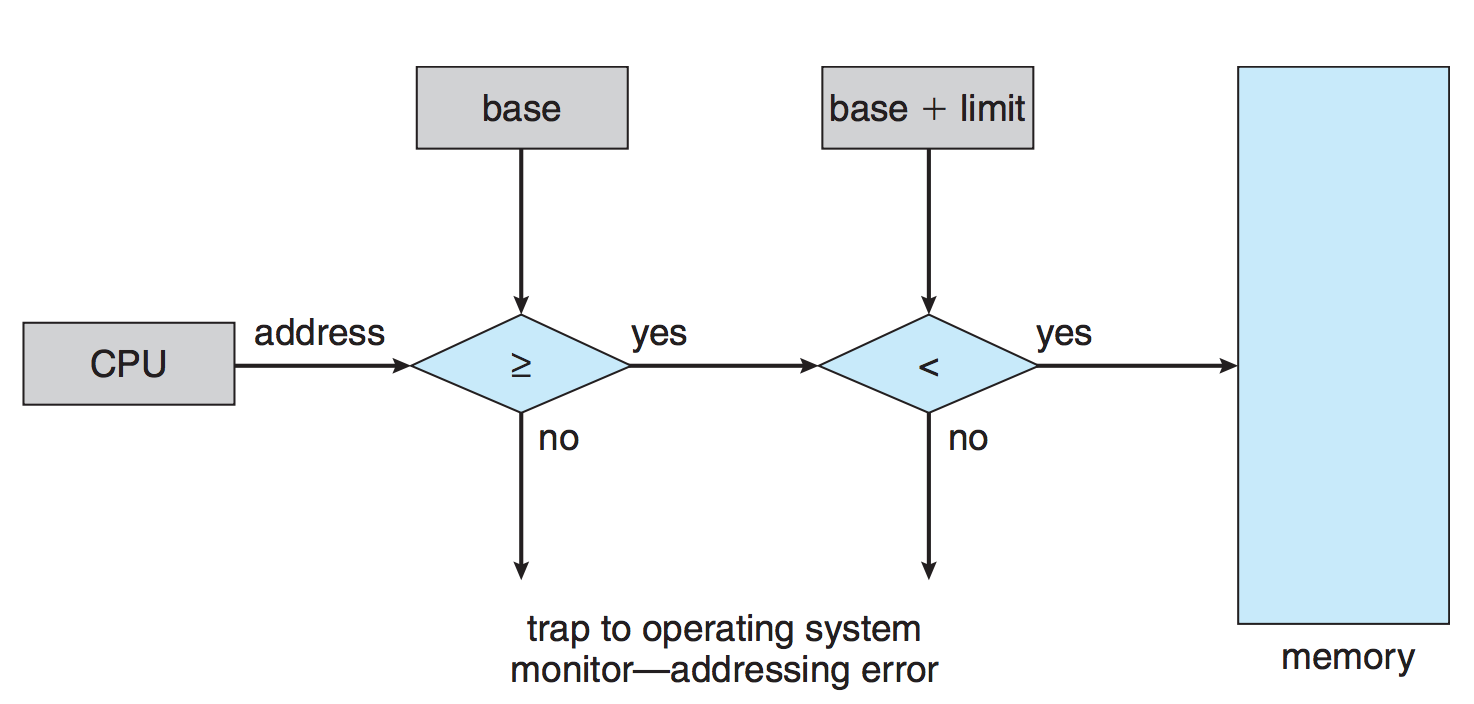
\includegraphics[width=0.7\textwidth]{images/memory-baselimit.png}\\
Hardware address protection with base and limit registers~\cite{osc}.
\end{center}


This, unfortunately, does not solve the problem. Imagine we have two programs numbers simply 1 and 2, each 16~KB in size. Suppose then we will load them into memory in different consecutive areas, as in the figure below:

\begin{center}
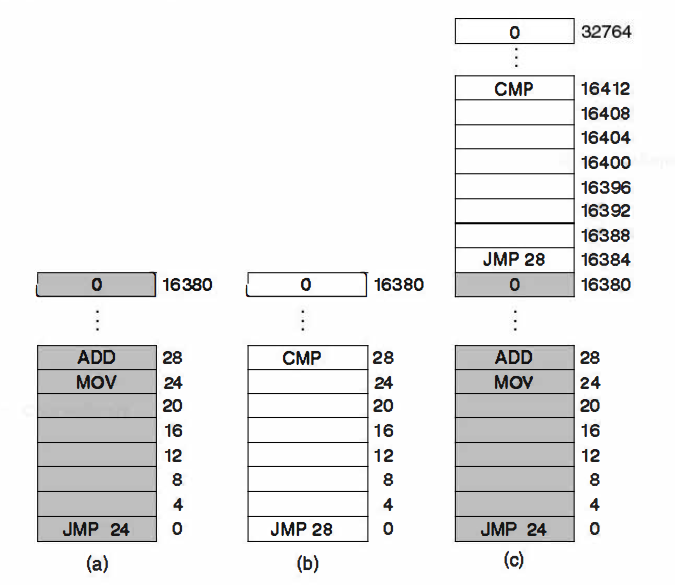
\includegraphics[width=0.70\textwidth]{images/os360.png}\\
(a) Program 1. (b) Program 2. (c) Programs 1 and 2 loaded into memory consecutively.~\cite{mos}.
\end{center}

Program 1 will execute as expected. The problem is immediately obvious when Program 2 runs. The instruction at address 16384 is executed: \texttt{JMP 28} takes execution to memory address 28 (an \texttt{ADD} instruction and not the expected address of 16412 and the \texttt{CMP} comparison). The problem is that both programs reference absolute physical locations. 

The IBM 360's stopgap solution to this was to do static relocation: if a program was being loaded to a base address 16384 the constant 16384 was added to every program address during the load process. While slow, if every address is updated correctly, the program works~\cite{mos}.

This is, unfortunately, not as easy as it sounds. A command like \texttt{JMP 28} must be relocated, but the 28 in a command like \texttt{ADD R1,28} (add 28 to register R1 and store the result in R1) is a constant and should not be changed. How do we know which is an address and which is a constant? It gets worse: in C a pointer contains an address, but addresses are just numbers, so in theory we could just dereference any integer variable and it would take us to a memory address (whether it's valid or not is not the point here). That makes it even harder to know if a number is just a number or an address.

When we are writing a program, unless it's in assembly, we do not usually refer to variables by their memory locations. The command we write looks something like \texttt{x = 5;} and although we know that variable \texttt{x} is stored in memory, the question arises: when is the variable assigned a location in memory? There are three obvious times to do it~\cite{osc}:

\begin{enumerate}
	\item \textbf{Compile time}: the solution we saw first with commands like \texttt{JMP 28}. If we are certain where the process will be loaded into memory, at compile time we can convert those variables to address locations. This is what happens in assembly, and in the MS-DOS .COM format (like \texttt{command.com}).
	\item \textbf{Load time}: the IBM 360 solution; at the time when the code is to be loaded into memory, the addresses are updated. This requires that the compiler indicate what numbers are addresses and should be updated when the program is loaded into memory.
	\item \textbf{Execution time}: if programs can move around in memory during execution (something we have not yet examined), then we need to do the binding at run-time. For this to work, though, we will need help from the hardware developers...
\end{enumerate}

\subsection*{Address Space}
It is clear that having no memory management system leaves us with a number of problems in memory. What we would like to do is introduce an abstraction; a layer of indirection. We do this with a concept called \textit{address space}. An address space is a set of addresses that a process can use; each process has its own address space, independent of other processes' address spaces (except when we create shared memory).

Telephone numbers in Canada and the USA take the form of NNN-NNNN, a seven digit number. In theory, any number in the range 000-0000 to 999-9999 could be issued, but in practice certain numbers are reserved (like the 000 or 555 prefixes). Given the number of telephones in the countries, seven digits could not possibly be enough (10 million numbers for a population around 350 million?!). In fact, many readers probably looked at this and thought it was wrong that phone numbers are seven digits; phone numbers are ten digits! Those three additional digits are the area code, after all, and they relate to a geographic area. The number 416-555-1234 is identifiable by its area code as being located in Toronto (or at least a cell phone registered there), and the number 212-555-1234 is in New York City. Although ten digit dialing is mandatory in Toronto (and presumably NYC), if you live in a district where ten digit dialing is not mandatory, you can dial 555-1234 and it will connect you to the number 555-1234 in your local area code. This is the idea we want to apply to memory: let each process have its own area code. So process can write to location 1024 and process 2 can write to location 1024 and these are two distinct locations, perhaps 21024 and 91024 respectively.

Now, instead of altering the addresses in memory, we will effectively prefix every memory access with an area code. The address that is generated by the CPU, e.g., the 28 in \texttt{JMP 28}, is the \textit{logical address}. We then add the area code to it to produce the \textit{physical address} (the actual location in memory and the address that it sent over the bus). In practice, to speed this up, it is done via some hardware, and the ``area code'' is a register called the \textit{relocation register} as below:

\begin{center}
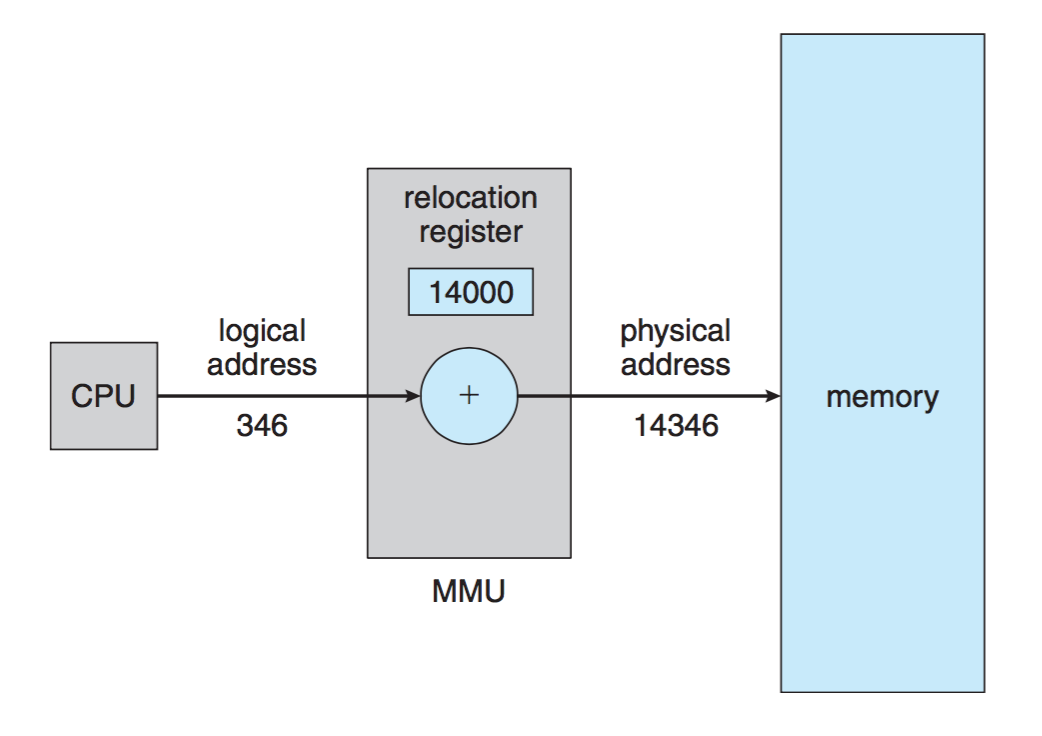
\includegraphics[width=0.5\textwidth]{images/relocation-register.png}\\
Dynamic translation of logical addresses to physical addresses with a relocation register~\cite{osc}.
\end{center}

The process itself does not know the physical address (14346 in the above example); it knows only the logical address (346). This is a run-time mapping of variables to memory.  We get some protection between processes, though we would get more protection if we brought back the limit register and compared the physical address to the base and [base + limit] values again. 

This scheme also gives us something new: we can relocate a process in memory if we change the relocation register's value accordingly. A process that is currently loaded into memory with a relocation register value of 14000 can easily be moved to another location. Copy all the memory from relocation register to the limit to a new location, such as 90000, and then update the relocation register to the new starting location (90000). After that, the old location of the process's memory can be marked as available or used by another process.

These benefits do not come for free. Every memory access now includes an addition (or two if the limit register comes into play). Comparisons are pretty quick for the CPU, but addition can be quite a bit slower, because of carry propagation time\footnote{If you are the sort of person who is really only interested in software and you have been wondering why the program has made you learn all sorts of details about hardware, this is a good example of why. You will have noticed in this section that the hardware developers have bailed the software developers out of various problems by taking operations that would be painfully slow and doing them a lot faster. In the case of the CPU addition carry propagation problem, if you don't understand the hardware, the software you write will be slow or problematic and you will not know why.}. So every memory access has a penalty associated with it to do the addition of the relocation register value to the issued CPU address. 

\subsection*{Swapping}

To run, a process must be in main memory. Given enough processes, or processes sufficiently demanding on the memory of the system, it will not be possible to keep all of them in memory at the same time. Processes that blocked may be taking up space in memory and it might be logical to make room for processes that are ready to run by moving blocked processes out of memory. The process of moving a process from memory to disk or vice-versa is called \textit{swapping}.

\begin{center}
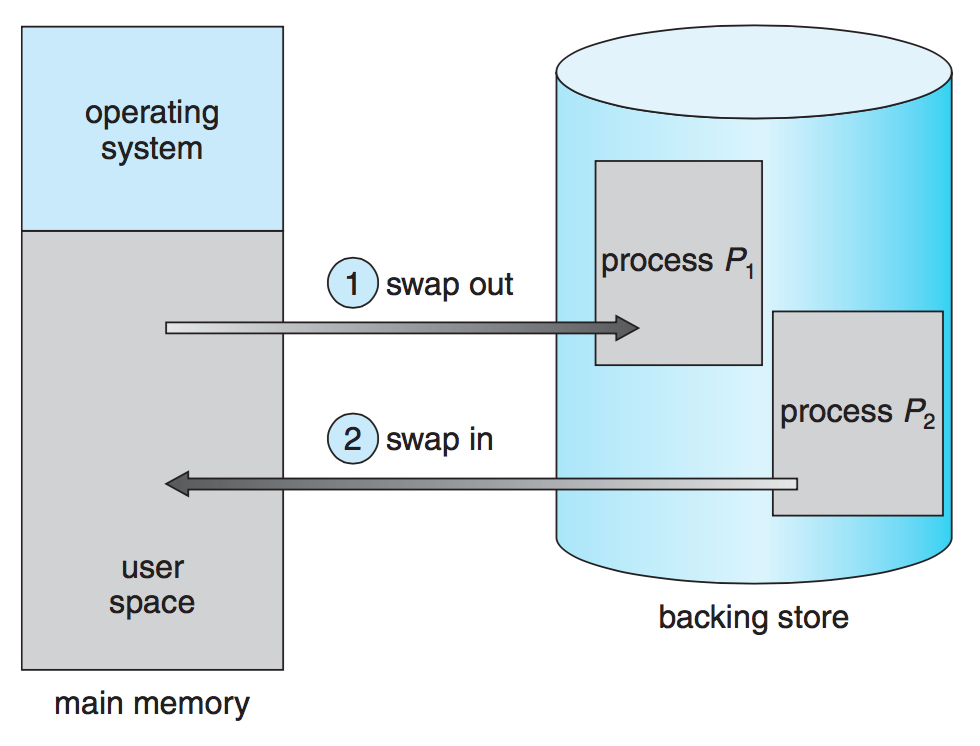
\includegraphics[width=0.5\textwidth]{images/swapping1.png}\\
Swapping processes (1) from memory to disk and (2) from disk to memory~\cite{osc}.
\end{center}

Unfortunately, swapping a process to disk is very painful. If the process is using 1~GB of memory, to swap a process out to disk, we need to write 1~GB of memory to disk. To load that process back later, it means reading another 1~GB from disk and putting it into main memory. If 1~GB strikes you as ridiculous in size, according to the Mac OS~X system utilities, with five PDF documents (whose combined file size on disk is 80.6~MB) open, the ``Preview'' application is consuming 2.05~GB as I write this. So, swapping is something we would like to do as little as possible, but it will be necessary eventually. 

Modern operating systems do not perform this kind of swapping because it is simply too slow. Too much time would be wasted swapping processes to and from disk. A modified form of swapping is used, but this is a subject we will return to later on in the examination of memory~\cite{osc}.

When swapping a process back in from disk it is not necessary to put it back in exactly the same place as it originally was. This works because the relocation register will be updated with the new location of the process when it is moved back to memory. See the diagram below showing the state of memory after seven swap operations.

\begin{center}
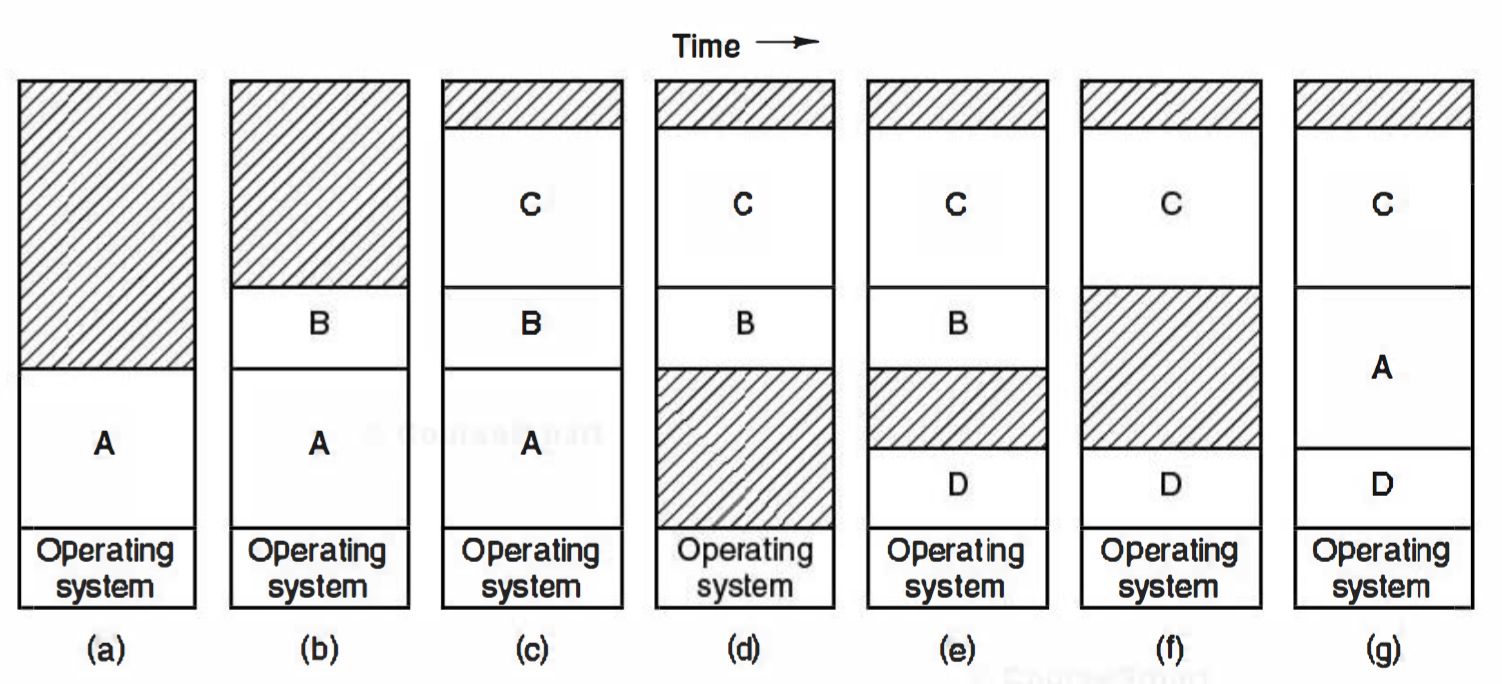
\includegraphics[width=0.8\textwidth]{images/swapping2.png}\\
A view of memory over time, swapping processes in and out as needed~\cite{mos}.
\end{center}

In (a), the only process in memory is $A$. In (b), process $B$ is added and in (c) process $C$ starts and is loaded into memory. When process $D$ would like to run, there is insufficient free space for it, so a process will need to be swapped out. In (d), process $A$ is chosen by the OS and is swapped out so that in (e) process $D$ may be in memory. If $A$ is ready to run again, space must be made for it, so $B$ is swapped out in (f) and then when $A$ is loaded the state of memory is as shown in (g).

Thus far we have considered process memory as a large, fixed-sized block. A process gets a big section of memory and operates in that area. As you know from previous programming experience, use of the \texttt{new} keyword in some languages, or \texttt{malloc()} in C, will result in dynamic memory allocation. We will have to deal with this next.

\bibliographystyle{alpha}
\bibliography{254}


\end{document}